%==============================================================================
% Template PROYECTO DE TITULO UCM
% Autor: Marco Quiroz
%        Escuela de Ing Civil
%        Departamento de Obras Civiles
%        Universidad Católica del Maule
%==============================================================================
\documentclass[12pt,letterpaper]{report}
\usepackage{UCM}
\usepackage{algorithm}
\usepackage{algpseudocode}
\floatname{algorithm}{Algorithme}
\algrenewcommand{\algorithmicrequire}{\textbf{Entrées :}}
\algrenewcommand{\algorithmicensure}{\textbf{Sorties :}}
\algrenewcommand{\algorithmicfor}{\textbf{pour}}
\algrenewcommand{\algorithmicdo}{\textbf{faire}}
\algrenewcommand{\algorithmicend}{\textbf{fin}}
\AtBeginDocument{\renewcommand*{\FrenchLabelItem}{\textnormal{-}}\renewcommand*{\Frlabelitemi}{\textnormal{-}}\renewcommand{\labelitemi}{\textnormal{-}}}
\captionsetup{labelsep=period}
\setlength{\emergencystretch}{3em}
\begin{document}
\hypersetup{pageanchor=false}
\pagestyle{empty}
\begin{center}
    \parbox[c][\textheight][t]{\textwidth}{
        \begin{center}
            \vspace*{1.5cm}
            
\includegraphics[width=0.42\textwidth]{logo/logo_cnam.png}\\
            \vspace{0.8cm}
            {\Large CONSERVATOIRE NATIONAL DES ARTS ET MÉTIERS}\\
            \vspace{0.25cm}
            {\large Master Finance de marché}\\
            \vspace{2.2cm}
            {\Large \bf L'approche agentique dans un contexte de trading multifactoriel}\\
            \vspace{0.75cm}
            {\large Synthèse LLM et allocation de portefeuille sous contraintes}\\
            \vspace{1.8cm}
            {\normalsize \bf Nom et prénom : SANOU Abou Dramane}\\
            {\normalsize \bf Encadrant : Bertrand DJEMBISSI}\\
            \vfill
            Rapport d'étude présenté dans le cadre du Master Finance de marché\\
            \vspace{0.5cm}
            Paris, septembre 2026
        \end{center}
        }
\end{center}

\cleardoublepage
%---------------------------------------------------------------------------
% Preamble
\hypersetup{pageanchor=true}
\pagenumbering{roman} 				% Begin Roman page numbering (i,ii,...)
% Résumé
\chapter*{Résumé}
 \addcontentsline{toc}{chapter}{Résumé}
Ce mémoire étudie deux usages d'un LLM en trading multifactoriel : restituer des résultats et proposer une allocation simulée sous contraintes. Le prototype initial associe un backtest Python, LangGraph et une synthèse DeepSeek. Dans l'extension, Python valide les poids proposés et calcule le portefeuille. Aucun outil d'ordre réel n'est accessible.

Quatre ETF représentent les expositions value, momentum, quality et low volatility : VLUE, MTUM, QUAL et USMV. Sur février 2015--décembre 2025, leur allocation équipondérée à 10 points de base atteint 12,02\,\% de rendement annualisé, contre 13,84\,\% pour SPY. Le contrôle temporel sur 2021--2025 conserve ce classement.

L'évaluation de la synthèse comprend 12 cas, dont 11 répétés trois fois et un cas qualité bloqué. Les 33 réponses passent les contrôles automatisés. Toutefois, trois altérations construites sont également acceptées : un coût nul, une citation inexistante et une recommandation contradictoire. La conformité mesurée ne garantit donc pas la fiabilité générale des notes.

L'extension d'allocation couvre mai 2021--décembre 2025 : 22 des 56 propositions sont exécutées et 34 rejetées, surtout pour dépassement du turnover. Pour 100 unités initiales, DeepSeek termine à 148,39, contre 153,55 pour l'équipondération et 152,26 pour l'inverse volatilité, après frais de transaction. Le replay reproduit ces résultats. Cette expérience rétrospective, exposée au biais de préentraînement et hors coûts API et humains, ne démontre pas d'avantage financier de l'agent.

\vspace{0.4cm}
\noindent \textbf{Mots-clés :} agents intelligents, trading multifactoriel, LLM, explicabilité, gouvernance, backtesting, LangGraph.

\clearpage
% Abstract
\chapter*{Abstract}
 \addcontentsline{toc}{chapter}{Abstract}
This report examines two uses of an LLM in multifactor trading: summarizing results and proposing constrained allocations in simulation. The initial prototype combines a Python backtest, LangGraph and a DeepSeek summary. In the extension, Python validates proposed weights and computes portfolio values. No live order tool is available.

Four ETFs represent value, momentum, quality and low volatility: VLUE, MTUM, QUAL and USMV. Over February 2015--December 2025, their equal-weighted portfolio with 10-basis-point transaction costs achieves a 12.02\% annualized return, versus 13.84\% for SPY. A temporal check over 2021--2025 preserves this ranking.

The summary evaluation covers 12 cases, including 11 repeated three times and one blocked data-quality case. All 33 responses pass automated checks. However, three constructed alterations also pass: a zero cost, a nonexistent citation and a contradictory recommendation. Measured compliance therefore does not guarantee general reliability.

The allocation extension covers May 2021--December 2025: 22 of 56 proposals are executed and 34 rejected, mainly for excessive turnover. Starting from 100 units, DeepSeek ends at 148.39, versus 153.55 for equal weighting and 152.26 for inverse volatility, after transaction costs. Archived replay reproduces these results. This retrospective experiment is exposed to pretraining look-ahead bias and excludes API and human costs; it does not establish a financial advantage for the agent.

\vspace{0.4cm}
\noindent \textbf{Keywords:} intelligent agents, multifactor trading, LLM, explainability, governance, backtesting, LangGraph.

\clearpage
% Remerciements
\chapter*{Remerciements}
\addcontentsline{toc}{chapter}{Remerciements}
Je remercie mon encadrant, Bertrand DJEMBISSI, pour son accompagnement et ses orientations dans la préparation de ce rapport d'étude. Je remercie également l'équipe pédagogique du CNAM pour le cadre de formation fourni au sein du Master Finance de marché.

\clearpage
\chapter*{Déclaration relative à l'utilisation de l'intelligence artificielle}
\addcontentsline{toc}{chapter}{Déclaration relative à l'utilisation de l'intelligence artificielle}
Dans le cadre de la préparation de ce rapport, j'ai utilisé des outils d'intelligence artificielle générative comme assistants de rédaction, de programmation et de vérification. Ils m'ont notamment aidé à corriger des fautes d'orthographe et de grammaire, à améliorer certaines formulations, à repérer des incohérences de notation et à vérifier la cohérence apparente de formules, de pseudo-codes et de portions de code. Cette assistance a également été mobilisée pour développer l'extension d'allocation, préparer ses tests, exécuter les simulations et rédiger leur analyse. Les contrôles automatisés et le replay sont documentés à partir du code, des équations et des archives ; ils ne valent pas validation indépendante de toutes les hypothèses financières. L'intelligence artificielle n'a donc pas été considérée comme une source autonome de résultats : les choix méthodologiques, l'analyse, l'interprétation et la validation finale présentés dans ce mémoire relèvent de ma responsabilité.

\cleardoublepage
%---------------------------------------------------------------------------
%The table of contents is automatically generated by the template
\setcounter{secnumdepth}{4}
\setcounter{tocdepth}{1}            % Sets the number of section levels in the table of contents to 4
\pagestyle{fancy}
\begingroup
\renewcommand{\baselinestretch}{1.1}\selectfont
\tableofcontents
\endgroup
\cleardoublepage                    % Ends the current page

\listoffigures
\addcontentsline{toc}{chapter}{\listfigurename}
\cleardoublepage
\begingroup
\renewcommand{\baselinestretch}{1.05}\small
\listoftables
\endgroup
\addcontentsline{toc}{chapter}{\listtablename}

\makeatletter
\@openrightfalse
\makeatother
\begingroup
\renewcommand{\baselinestretch}{1.05}\selectfont

\newacronym{ia}{IA}{intelligence artificielle}
\newacronym{llm}{LLM}{grand modèle de langage}
\newacronym{rag}{RAG}{génération augmentée par récupération}
\newacronym{rl}{RL}{apprentissage par renforcement}
\newacronym{api}{API}{interface de programmation applicative}
\newacronym{etf}{ETF}{fonds indiciel coté}
\newacronym{var}{VaR}{valeur en risque}
\newacronym{es}{ES}{expected shortfall}
\newacronym{pnl}{PnL}{profit and loss}
\newacronym{mifid}{MiFID II}{Markets in Financial Instruments Directive II}
\newacronym{dora}{DORA}{Digital Operational Resilience Act}
\newacronym{mar}{MAR}{Market Abuse Regulation}
\newacronym{hft}{HFT}{trading haute fréquence}
\newacronym{humanloop}{HITL}{human-in-the-loop}

% Acronymes d'exemple du template conservés hors compilation.
%
\let\cleardoublepage\clearpage
\printglossary[type=\acronymtype,title=Glossaire, toctitle=Glossaire]
%\addcontentsline{toc}{chapter}{Glossaire}
\glsaddallunused
%\glsaddall

\endgroup
\makeatletter
\@openrighttrue
\makeatother
\cleardoublepage

% Chapitres
\pagestyle{fancy}               	% Fancy headings
\pagenumbering{arabic}				% Begin arabic page numbering (1,2,...)
\setlength{\parindent}{20pt}        % Sets default paragraph indentation to 20 pt

\clearpage

% Chapitres
\chapter{Introduction et problématique}\label{cap:introduction}
%--------------------------------------

\section{Contexte général}

Le trading multifactoriel consiste à construire des décisions d'investissement à partir de plusieurs familles de signaux : valorisation, momentum, qualité, faible volatilité, liquidité, portage, révisions d'analystes, signaux macroéconomiques ou signaux issus de nouvelles. Cette logique prolonge la tradition académique des modèles factoriels, depuis les facteurs de marché, taille et valeur de \citet{famaFrench1993} jusqu'au facteur momentum formalisé par \citet{carhart1997}. Dans un contexte professionnel, ces facteurs ne suffisent pas à eux seuls : ils doivent être nettoyés, normalisés, neutralisés, testés hors échantillon, combinés avec des contraintes de risque, puis traduits en ordres compatibles avec la liquidité et le mandat du portefeuille.

Les avancées récentes des grands modèles de langage ont introduit une nouvelle brique dans cette chaîne. Un agent ne se limite pas à produire du texte : il peut appeler des outils, lire des documents, interroger une base de données, déléguer des tâches à d'autres agents et enregistrer les raisons d'une décision. Les travaux sur ReAct \citep{yao2023react}, Toolformer \citep{schick2023toolformer}, Reflexion \citep{shinn2023reflexion} et AutoGen \citep{wu2023autogen} ont montré que le raisonnement, l'utilisation d'outils et l'interaction multi-agents peuvent être assemblés en workflows plus robustes qu'un simple prompt isolé.

Pour un desk de trading, cette évolution ouvre des cas d'usage concrets : veille de marché, qualification de nouvelles, synthèse de recherche, génération de scénarios, préparation de revues de risque, documentation des décisions, contrôle de cohérence d'une stratégie et assistance au backtesting. En revanche, elle ne supprime pas les exigences fondamentales de la finance de marché : contrôle du risque, séparation des responsabilités, validation indépendante, explicabilité, auditabilité et surveillance continue.

\section{Problématique}

La question centrale de ce rapport est la suivante : comment utiliser une approche agentique dans un environnement de trading multifactoriel sans transformer un outil d'aide à la décision en boîte noire opérationnelle ? Cette question est plus exigeante que la simple automatisation d'un script de trading. Un agent fondé sur un LLM peut produire une justification plausible sans que cette justification soit causalement liée au signal réellement utilisé. Il peut aussi confondre une corrélation historique avec une relation exploitable, ignorer une limite de risque ou synthétiser une nouvelle de marché sans mesurer son impact probabiliste.

Le domaine est fortement réglementé. En Europe, les exigences relatives au trading algorithmique imposent des systèmes résilients, des contrôles de risque et des limites permettant d'éviter des conditions de marché désordonnées \citep{mifidArticle17}. Le règlement DORA renforce les obligations liées au risque informatique et à la résilience opérationnelle des entités financières \citep{dora2022}. Les cadres de gestion des risques liés à l'IA, comme le NIST AI Risk Management Framework, insistent sur la gouvernance, la mesure, la cartographie des risques et le monitoring \citep{nistAirmf2023}. Même lorsque l'usage n'entre pas automatiquement dans une catégorie d'IA à haut risque au sens de l'AI Act \citep{euAiAct2024}, les principes de contrôle, de documentation et de surveillance restent indispensables dans une institution financière.

La problématique peut donc être formulée ainsi : quelles architectures agentiques disponibles aujourd'hui, notamment sur GitHub, peuvent contribuer à un desk de trading multifactoriel explicable, rationnel et monitorable, et quelles limites empêchent encore leur déploiement autonome en production ?

\section{Objectifs du rapport}

Ce rapport poursuit cinq objectifs :
\begin{enumerate}
    \item établir un état de l'art des architectures agentiques pertinentes pour la finance de marché ;
    \item recenser les projets GitHub qui peuvent être mobilisés pour analyser l'état actuel des architectures agentiques en finance de marché ;
    \item comparer ces projets selon des critères observables : gestion de l'état, persistance, supervision humaine, permissions d'outils, reprise après incident, mémoire, backtesting et traçabilité ;
    \item proposer une architecture cible dans laquelle les agents assistent la décision sans remplacer les contrôles quantitatifs et humains nécessaires ;
    \item expérimenter un socle quantitatif et une couche agentique supervisée afin d'évaluer la reproductibilité des calculs, la fidélité des synthèses et le respect des permissions.
\end{enumerate}

\section{Périmètre}

Le rapport se concentre sur les actions liquides, ETF, futures et crypto-actifs comme univers d'étude pour les solutions ouvertes. Les produits complexes, l'optimisation fiscale, le trading haute fréquence et les infrastructures propriétaires d'exécution ne sont pas étudiés en détail.

Le travail ne vise pas à construire une plateforme de trading prête pour la production, à démontrer une capacité à générer de l'alpha ou à proposer un dispositif réglementaire complet. Il valide certains principes architecturaux à travers un prototype expérimental : séparation entre calcul et interprétation, contrôle hors échantillon, journalisation structurée, permissions limitées et validation humaine. Les résultats financiers sont donc des résultats de démonstration et non une recommandation d'investissement.

L'analyse distingue trois niveaux :
\begin{description}
    \item[Agents généralistes :] frameworks permettant de coordonner des rôles, outils, mémoires et workflows.
    \item[Briques quantitatives :] bibliothèques de données, backtesting, recherche factorielle, apprentissage par renforcement et exécution simulée.
    \item[Applications financières agentiques :] dépôts combinant LLM, analyse financière et décision d'investissement.
\end{description}

\section{Organisation du rapport}

Le chapitre~\ref{cap:etat-art} présente l'état de l'art et la cartographie des solutions GitHub. Le chapitre~\ref{cap:methodologie} décrit la méthode de sélection et d'évaluation. Le chapitre~\ref{cap:architecture} propose une architecture cible multi-agents adaptée au trading multifactoriel. Le chapitre~\ref{cap:discussion} discute les risques, les limites et les conditions de mise en production. Le chapitre~\ref{cap:conclusion} conclut et propose des pistes d'approfondissement.

% Texte d'exemple du template conservé hors compilation.


\chapter{État de l'art et choix des composants}\label{cap:etat-art}

\section{Définir l'approche agentique}

Dans ce mémoire, le terme « agentique » désigne l'organisation de tâches autour d'un état partagé, d'outils et de règles de passage entre étapes. Le prototype initial en retient une forme limitée : LangGraph coordonne les contrôles et les traitements déterministes, puis peut déclencher une synthèse DeepSeek. Il ne s'agit pas d'une équipe autonome d'agents financiers.

J'ai retenu de ReAct et de Toolformer l'usage d'outils externes pour fournir au modèle les résultats dont il a besoin \citep{yao2023react,schick2023toolformer}. Dans mon cas d'usage, les rendements, les coûts et les autres valeurs financières sont calculés en amont, puis transmis au modèle. Le RAG pourrait compléter cette architecture pour traiter des documents ou des actualités financières \citep{lewis2020rag}, mais il n'est pas utilisé dans l'expérience.

Reflexion et AutoGen apportent des pistes pour l'architecture cible, avec le retour critique ou les échanges entre agents \citep{shinn2023reflexion,wu2023autogen}. Ces mécanismes dépassent le besoin de l'expérience initiale de synthèse : le LLM y restitue un état quantitatif déjà produit. Il ne calcule pas le signal, dont la robustesse doit être évaluée séparément de la qualité de la synthèse.


\section{Du besoin du prototype au choix des outils}

La comparaison de LangGraph et de Lean m'a aidé à séparer deux besoins : organiser les étapes d'un workflow et simuler un portefeuille \citep{githubLangGraph,githubLean}. J'ai conservé un moteur Python pour les calculs de quatre ETF, puis LangGraph pour suivre l'état et bloquer la synthèse si le contrôle qualité échoue. Les autres frameworks ont été comparés sur documents, sans essai d'exécution permettant de les classer en performance.

Le tableau~\ref{tab:frameworks-agents} situe les six frameworks examinés. Le choix de LangGraph repose sur les transitions et le suivi de l'état mobilisés dans mon prototype ; les calculs et les règles métier sont des fonctions séparées.

\begin{table}[H]
\centering
\caption{Frameworks agentiques généralistes disponibles sur GitHub.}
\label{tab:frameworks-agents}
\scriptsize
\begin{adjustbox}{width=\textwidth}
\begin{tabular}{p{0.18\textwidth}p{0.24\textwidth}p{0.30\textwidth}p{0.24\textwidth}}
\toprule
\textbf{Projet GitHub} & \textbf{Positionnement} & \textbf{Intérêt pour un desk multifactoriel} & \textbf{Limites principales} \\
\midrule
LangGraph \citep{githubLangGraph} & Workflows d'agents sous forme de graphes, avec état persistant et contrôle fin des transitions. & Adapté aux processus audités : ingestion, calcul de facteurs, revue de risque, validation, journalisation. & Nécessite de développer les outils quantitatifs et les contrôles métier autour du graphe. \\
AutoGen \citep{githubAutoGen} & Conversations multi-agents et orchestration d'équipes d'agents. & Utile pour comparer des rôles de recherche, analyste, contrôleur de risque et superviseur. & Les conversations libres doivent être fortement contraintes pour un usage régulé. \\
CrewAI \citep{githubCrewAI} & Agents orientés rôles, tâches et processus. & Simple pour construire une équipe d'agents de recherche de marché et de reporting. & Moins adapté seul aux workflows critiques nécessitant des états vérifiables et des garde-fous stricts. \\
Semantic Kernel \citep{githubSemanticKernel} & SDK Microsoft pour connecter modèles, plugins, fonctions et mémoire. & Intéressant dans un environnement d'entreprise déjà Microsoft, avec intégration possible à des services internes. & L'architecture de trading reste à construire ; le framework ne fournit pas de modèle financier. \\
CAMEL \citep{githubCamel} & Environnements et méthodes pour sociétés multi-agents. & Pertinent pour expérimenter des interactions entre analystes spécialisés. & Plus orienté recherche agentique que production financière. \\
OpenAI Swarm \citep{githubSwarm} & Exemple éducatif de routage entre agents. & Montre clairement la logique de transfert entre rôles. & Projet expérimental, insuffisant pour une architecture de production. \\
\bottomrule
\end{tabular}
\end{adjustbox}
\end{table}

\section{Socle quantitatif et accès aux données}

Une recherche sur actions individuelles demanderait de définir l'univers, préparer les données, calculer les signaux et construire le portefeuille sous contraintes. J'ai réduit ce travail à VLUE, MTUM, QUAL et USMV, initialement équipondérés et rééquilibrés chaque mois. Les ETF représentent les expositions ; le prototype ne reconstruit pas les facteurs titre par titre. L'extension d'allocation conserve cet univers et compare les propositions DeepSeek à deux règles simples.

\begin{table}[H]
\centering
\caption{Briques quantitatives GitHub utiles pour une étude multifactorielle.}
\label{tab:github-quant}
\scriptsize
\begin{adjustbox}{width=\textwidth}
\begin{tabular}{p{0.18\textwidth}p{0.25\textwidth}p{0.32\textwidth}p{0.21\textwidth}}
\toprule
\textbf{Projet GitHub} & \textbf{Fonction principale} & \textbf{Apport dans l'architecture cible} & \textbf{Point d'attention} \\
\midrule
Qlib \citep{githubQlib} & Plateforme Microsoft orientée recherche quantitative, données, modèles et backtesting. & Bon socle pour tester des facteurs, pipelines de données et modèles prédictifs. & Adaptation nécessaire aux données internes et aux contraintes de portefeuille réelles. \\
FinRL \citep{githubFinRL} et FinRL-Meta \citep{githubFinRLMeta} & Apprentissage par renforcement pour trading automatisé et environnements de marché. & Utile pour comparer une approche agentique LLM avec des agents RL plus classiques. & Le RL financier souffre fortement du surapprentissage et des coûts de transaction mal modélisés. \\
FinRL-X \citep{finrlx2026} & Infrastructure modulaire récente pour trading quantitatif natif IA. & Référence pour étudier l'intégration des briques de trading dans une infrastructure modulaire. & Projet récent : maturité opérationnelle à vérifier avant usage critique. \\
QuantConnect Lean \citep{githubLean} & Moteur open source de backtesting et trading algorithmique multi-actifs. & Brique robuste pour simuler et exécuter des stratégies dans un cadre contrôlé. & L'agent doit rester au-dessus du moteur, sans contourner les règles d'exécution. \\
OpenBB \citep{githubOpenBB} & Plateforme ouverte d'accès aux données et analyses financières. & Source pratique pour créer un agent de recherche et de veille. & La qualité dépend des fournisseurs de données configurés et de leurs licences. \\
Freqtrade \citep{githubFreqtrade} & Bot de trading crypto avec backtesting et hyperoptimisation. & Utile pour une étude sur crypto-actifs, où l'accès aux données et exchanges est simple. & Domaine crypto moins représentatif des contraintes actions institutionnelles. \\
\bottomrule
\end{tabular}
\end{adjustbox}
\end{table}

Qlib aurait répondu à un besoin de comparaison de modèles prédictifs ou de pipelines de facteurs. Mon expérience n'apprend pas de modèle et part de quatre ETF : j'ai conservé un moteur Python plus simple. Lean reste une référence pour une simulation multi-actifs plus complète. OpenBB a surtout été étudié pour l'agent de veille proposé ; le backtest disposait déjà de son historique. Une intégration d'actualités demanderait de documenter leur provenance, leur licence et leur disponibilité à la date de décision.

\section{Projets financiers et enseignements retenus}

\begin{table}[H]
\centering
\caption{Solutions GitHub orientées agents financiers.}
\label{tab:github-finance-agents}
\scriptsize
\begin{adjustbox}{width=\textwidth}
\begin{tabular}{p{0.18\textwidth}p{0.27\textwidth}p{0.31\textwidth}p{0.20\textwidth}}
\toprule
\textbf{Projet GitHub} & \textbf{Principe} & \textbf{Ce qu'il apporte au sujet} & \textbf{Limite pour un desk régulé} \\
\midrule
TradingAgents \citep{githubTradingAgents} & Framework multi-agents imitant une société de trading avec analystes spécialisés, trader et gestion du risque. & C'est l'un des dépôts les plus proches de l'idée d'équipe multi-agents appliquée au trading. & À analyser comme démonstrateur de recherche ; il faut ajouter validation des données, limites de risque, audit et contrôle humain. \\
FinRobot \citep{githubFinRobot} & Plateforme d'agents LLM pour applications financières, notamment recherche actions, analyse et valorisation. & Automatisation de tâches d'analyse financière et de rédaction de synthèses structurées. & Plus orienté analyse et reporting que génération robuste d'ordres multifactoriels. \\
FinMem \citep{finmem2023,githubFinMem} & Agent de trading fondé sur mémoire stratifiée et profils de décision. & Montre l'intérêt de la mémoire long terme pour contextualiser les décisions de trading. & Les performances expérimentales ne suffisent pas à prouver une robustesse exploitable en production. \\
AI Hedge Fund \citep{githubAiHedgeFund} & Démonstrateur open source d'un fonds simulé composé d'agents d'investissement. & Le dépôt illustre une répartition des tâches entre agents d'analyse et agent de décision. & Le dépôt se présente comme preuve de concept, pas comme outil de trading réel. \\
FinGPT \citep{fingpt2023,githubFinGPT} & Écosystème de modèles de langage financiers open source. & Modèles financiers à intégrer ou adapter pour des tâches d'analyse spécialisées. & Un modèle financier n'est pas une architecture de décision ; il faut ajouter outils, gouvernance et backtesting. \\
\bottomrule
\end{tabular}
\end{adjustbox}
\end{table}

TradingAgents et FinRobot ont nourri deux aspects du projet : la séparation des rôles d'analyse et de risque, puis les tâches de reporting proches de la note étudiée. FinMem soulève la question des synthèses passées : les conserver pourrait apporter du contexte, mais aussi transmettre leurs erreurs aux décisions suivantes. Cette mémoire reste hors du prototype. Aucun des cinq projets financiers n'a été exécuté ; leurs performances ne sont donc pas comparées à celles du backtest.

\section{Statut des briques et portée de la revue}

LangGraph est utilisé dans le workflow de restitution. Qlib, Lean et OpenBB sont des références étudiées, sans participation aux calculs finaux. TradingAgents et FinRobot ont inspiré les rôles proposés ; FinRL et Freqtrade relèvent d'autres périmètres expérimentaux. Pour examiner les dépôts, j'ai regardé l'état, les transitions, les permissions, la persistance, la documentation et les tests. La due diligence datée des huit dépôts retenus figure en annexe~\ref{annexe:github}.

La revue a conduit à un cas que je pouvais vérifier à partir des artefacts produits : confronter une réponse DeepSeek aux chiffres sources et à une note déterministe. L'extension mesure ensuite les conséquences de poids proposés sur le PnL. Les interactions libres entre agents et la mémoire ne font pas partie de ces expériences.

Les articles scientifiques étayent les concepts et les résultats ; les textes officiels éclairent la gouvernance. Les prépublications sont signalées comme telles. Les dépôts et documentations décrivent les fonctionnalités et les conditions d'intégration. Google Scholar, ScienceDirect et JSTOR ont servi au repérage ; les références renvoient autant que possible à l'article original, au DOI ou à une version légale déposée.


\chapter{Méthodologie d'analyse}\label{cap:methodologie}
%--------------------------------------

\section{Démarche documentaire}

L'état de l'art a été construit à partir de trois types de sources. Les sources académiques servent à comprendre les concepts : agents LLM, raisonnement avec outils, génération augmentée par récupération, mémoire, collaboration multi-agents et modèles factoriels. Les sources réglementaires servent à fixer les contraintes minimales d'un contexte financier : contrôle du trading algorithmique, résilience opérationnelle, gouvernance du risque IA et auditabilité. Enfin, les dépôts GitHub servent à identifier les solutions réellement disponibles et leur degré de maturité. Lorsque les documents étaient librement accessibles en PDF, ils ont été archivés dans le sous-dossier \texttt{papers} afin de constituer un corpus documentaire local. Les articles soumis à licence éditeur restent cités en bibliographie sans copie locale.

La recherche GitHub a été structurée autour de mots-clés : \emph{LLM agent trading}, \emph{multi-agent financial trading}, \emph{financial LLM agent}, \emph{quantitative trading framework}, \emph{backtesting engine}, \emph{FinRL}, \emph{Qlib}, \emph{OpenBB}, \emph{LangGraph}, \emph{AutoGen} et \emph{CrewAI}. Les dépôts retenus devaient satisfaire au moins l'un des critères suivants :

\begin{itemize}
    \item fournir une brique d'orchestration agentique ;
    \item traiter explicitement un cas d'usage financier ;
    \item fournir une infrastructure utile au trading multifactoriel : données, backtesting, moteur d'exécution simulée, apprentissage par renforcement ou recherche quantitative ;
    \item rendre le code accessible publiquement pour étude, adaptation ou expérimentation.
\end{itemize}

Le corpus de comparaison comprend 17 fiches : 6 frameworks généralistes, 6 briques quantitatives et 5 projets spécifiquement financiers. Huit dépôts ont ensuite été retenus pour la due diligence finale, tandis que les autres ont été conservés comme références comparatives ou écartés du prototype. Ce décompte porte sur les fiches étudiées et non sur une mesure exhaustive de tous les dépôts repérés. Les dépôts trop éloignés du sujet, purement marketing, sans code exploitable ou uniquement centrés sur des signaux isolés ont été écartés. Les informations sur GitHub doivent être réévaluées avant toute mise en production, car l'activité, la licence, les dépendances et les mainteneurs peuvent évoluer rapidement.

\section{Revue réglementaire arrêtée au 30 août 2026}

Cette revue est documentaire et ne constitue pas un avis juridique. Elle sert à relier l'architecture proposée aux sources officielles disponibles à la date d'arrêté.

\begin{itemize}
    \item \textbf{MiFID II, article 17 :} le trading algorithmique implique des systèmes et contrôles de risque adaptés, des limites, des tests et une capacité à décrire les paramètres et contrôles à l'autorité compétente \citep{mifidArticle17}.
    \item \textbf{DORA :} le règlement (UE) 2022/2554 s'applique depuis le 17 janvier 2025 et renforce la résilience opérationnelle numérique des entités financières \citep{dora2022}.
    \item \textbf{AI Act :} le règlement (UE) 2024/1689 s'applique en principe depuis le 2 août 2026, avec des dates spécifiques pour certaines dispositions, notamment le 2 février 2025, le 2 août 2025 et le 2 août 2027 \citep{euAiAct2024}. L'applicabilité à un système donné dépend de son usage et de son rôle juridique.
    \item \textbf{NIST AI RMF :} le référentiel AI RMF 1.0 fournit une base de gouvernance, de cartographie, de mesure et de gestion des risques ; la page officielle indique qu'une révision est en cours \citep{nistAirmf2023}.
\end{itemize}

La conséquence opérationnelle est claire : toute mise en production requiert une validation séparée par les fonctions risque, conformité, juridique et IT. Les références ci-dessus doivent être relues à chaque changement de périmètre, de modèle, de fournisseur ou de régime réglementaire.

\section{Grille d'évaluation et scoring}

La grille compare les solutions sans confondre popularité open source et aptitude à un environnement de marché régulé. Chaque critère reçoit une note de 0 à 3 :

\begin{itemize}
    \item 0 : critère absent ou impossible à vérifier dans les sources publiques ;
    \item 1 : élément partiel, seulement illustré ou nécessitant un développement important ;
    \item 2 : capacité documentée et utilisable avec une adaptation maîtrisée ;
    \item 3 : capacité explicite, testable et directement intégrable dans un workflow contrôlé.
\end{itemize}

\begin{table}[H]
\centering
\caption{Grille de scoring des solutions agentiques et quantitatives.}
\label{tab:grille-evaluation}
\scriptsize
\begin{adjustbox}{width=\textwidth}
\begin{tabular}{p{0.18\textwidth}p{0.31\textwidth}p{0.27\textwidth}p{0.18\textwidth}}
\toprule
\textbf{Critère} & \textbf{Question d'évaluation} & \textbf{Barème 0-3} & \textbf{Interprétation} \\
\midrule
Couverture fonctionnelle & Le projet couvre-t-il orchestration, données, backtest, risque, exécution ou reporting ? & 0 absent ; 1 partiel ; 2 plusieurs fonctions ; 3 chaîne cohérente & Mesure l'étendue, sans assimiler étendue et maturité. \\
Reproductibilité & Les calculs et décisions peuvent-ils être rejoués avec les mêmes données et paramètres ? & 0 non vérifiable ; 1 exemples ; 2 pipeline documenté ; 3 tests et versionnement & Condition de base pour audit et validation. \\
Explicabilité & Les sorties relient-elles la justification aux signaux, sources et contraintes ? & 0 aucune ; 1 texte libre ; 2 sorties structurées ; 3 preuve liée aux données & Distingue une narration plausible d'une explication vérifiable. \\
Contrôle du risque & Existe-t-il des limites, validations, stress tests ou garde-fous ? & 0 absent ; 1 implicite ; 2 documenté ; 3 bloquant et testé & Critère critique avant toute exécution. \\
Qualité logicielle & Le dépôt propose-t-il documentation, tests, exemples et structure maintenable ? & 0 absent ; 1 incomplet ; 2 présent ; 3 intégré et suivi & Réduit le risque opérationnel. \\
Intégrabilité & Le projet s'interface-t-il avec Python, bases, API ou moteurs de backtesting ? & 0 isolé ; 1 adaptation forte ; 2 interfaces disponibles ; 3 intégration directe & Détermine la faisabilité d'une architecture composée. \\
Gouvernance & Les rôles, permissions, journaux et validations sont-ils explicitement modélisés ? & 0 absent ; 1 déclaratif ; 2 partiel ; 3 contrôlable et auditable & Indispensable dans une institution financière. \\
\bottomrule
\end{tabular}
\end{adjustbox}
\end{table}

Le score maximal est de 21 points. Les notes ci-dessous sont une lecture documentaire provisoire des dépôts retenus ; elles ne constituent ni une certification, ni une validation de production. Elles servent à rendre visibles les arbitrages effectués dans le mémoire.

\begin{table}[H]
\centering
\caption{Scoring documentaire provisoire des dépôts retenus.}
\label{tab:scoring-depots}
\scriptsize
\begin{adjustbox}{width=\textwidth}
\begin{tabular}{lrrrrrrrr}
\toprule
\textbf{Dépôt} & \textbf{Couverture} & \textbf{Reprod.} & \textbf{Explic.} & \textbf{Risque} & \textbf{Qualité} & \textbf{Intégr.} & \textbf{Gouv.} & \textbf{Total} \\
\midrule
LangGraph & 2 & 3 & 2 & 1 & 3 & 3 & 2 & 16/21 \\
Qlib & 3 & 3 & 1 & 1 & 3 & 3 & 1 & 15/21 \\
Lean & 3 & 3 & 1 & 2 & 3 & 3 & 1 & 16/21 \\
OpenBB & 2 & 2 & 1 & 0 & 3 & 3 & 1 & 12/21 \\
TradingAgents & 2 & 1 & 2 & 0 & 2 & 2 & 1 & 10/21 \\
FinRobot & 2 & 1 & 2 & 0 & 2 & 2 & 1 & 10/21 \\
FinRL & 2 & 2 & 1 & 1 & 2 & 2 & 1 & 11/21 \\
Freqtrade & 3 & 2 & 1 & 1 & 3 & 3 & 1 & 14/21 \\
\bottomrule
\end{tabular}
\end{adjustbox}
\end{table}

Le tableau confirme le choix d'une architecture composée. LangGraph obtient son meilleur niveau sur l'orchestration et l'intégrabilité, tandis que Qlib et Lean sont plus solides pour la recherche et le backtesting. Les scores de gouvernance et de contrôle du risque restent faibles ou partiels, ce qui justifie l'ajout de règles métier externes et d'une validation humaine.

\section{Principes de conception}

Ces principes ne sont pas des hypothèses statistiques. Ils fixent les règles de conception qui relient le socle quantitatif, la couche agentique et la gouvernance :

\begin{description}
    \item[Séparation du calcul et de l'interprétation :] les facteurs, rendements, pondérations, coûts et indicateurs de risque sont calculés par des fonctions déterministes. L'agent lit ces sorties, les contrôle et les explique sans les réécrire.
    \item[Supervision humaine :] une recommandation agentique est un objet de revue. Toute action engageant le portefeuille, et notamment l'envoi d'un ordre, reste soumise à une validation explicite et à des permissions indépendantes.
    \item[Explicabilité vérifiable :] une justification doit renvoyer aux données, aux versions, aux contraintes et aux règles réellement utilisées. Le texte produit ne remplace pas le journal structuré.
\end{description}

\section{Méthode de classement des solutions}

Chaque projet est classé selon son rôle principal :

\begin{description}
    \item[Orchestration :] organisation des agents, des tâches, de l'état et des outils.
    \item[Recherche financière :] collecte, résumé et analyse d'informations financières.
    \item[Infrastructure quantitative :] calcul de signaux, backtesting, environnement de simulation ou moteur d'exécution.
    \item[Gouvernance :] capacité à tracer, valider, surveiller et expliquer les décisions.
\end{description}

Cette classification évite une erreur fréquente : comparer un framework agentique comme LangGraph à un moteur de backtesting comme Lean. Les deux sont complémentaires. Dans une architecture cible, LangGraph peut piloter le workflow, Qlib calculer des signaux, OpenBB fournir des données, Lean simuler l'exécution, et un agent spécialisé produire un rapport de décision.

\section{Protocole expérimental}

Un prototype quantitatif minimal a été ajouté afin de tester le socle déterministe de l'architecture proposée. Le but n'est pas de démontrer qu'un agent ou une stratégie produit systématiquement de l'alpha, mais de vérifier que les données, les calculs de portefeuille, les coûts et les indicateurs de risque peuvent être rejoués de manière reproductible avant toute intervention d'un agent de synthèse.

Le protocole utilise quatre ETF factoriels américains comme proxies investissables de sleeves de valeur, momentum, qualité et faible volatilité : \texttt{VLUE}, \texttt{MTUM}, \texttt{QUAL} et \texttt{USMV}. Ces ETF ne constituent pas une reconstruction titre par titre des facteurs value, momentum, quality et low volatility : ils servent de portefeuilles observables représentant ces expositions. Le benchmark est \texttt{SPY}. Les cours ajustés sont téléchargés via \texttt{yfinance} \citep{yfinance} sur la période allant du 1er janvier 2015 au 31 décembre 2025. Le portefeuille multifactoriel est équipondéré et rééquilibré à la fin de chaque mois.

Trois hypothèses de coûts de transaction sont testées : 0, 10 et 30 points de base par unité de turnover. Le taux sans risque est fixé à 0\,\% pour faciliter la comparaison du ratio de Sharpe. Les indicateurs calculés sont le rendement annualisé, la volatilité annualisée, le ratio de Sharpe, le maximum drawdown, la valeur finale d'un investissement initial de 100 unités et le turnover.

Pour un mois $t$, le rendement net du portefeuille est calculé selon :
\[
r_t^{\mathrm{net}} = \sum_i w_{i,t-1}r_{i,t} - c\tau_t,
\qquad
\tau_t = \frac{1}{2}\sum_i\left|w_{i,t}-w_{i,t-1}\right|,
\]
où $c$ désigne le coût unitaire exprimé en fraction et $\tau_t$ le turnover au rebalancement. Sur $T$ rendements mensuels, les métriques principales sont :
\[
R_{\mathrm{ann}} = \left(\prod_{t=1}^{T}(1+r_t)\right)^{12/T}-1,
\qquad
\sigma_{\mathrm{ann}} = \sqrt{12}\,\mathrm{sd}(r_t),
\qquad
S = \frac{R_{\mathrm{ann}}}{\sigma_{\mathrm{ann}}}.
\]
Le drawdown est obtenu à partir du rapport entre la valeur courante et le maximum historique de la valeur cumulée. Ces formules rendent explicite le traitement des coûts, du turnover et de l'annualisation.

Le déroulement peut être résumé par le pseudo-code suivant :

\begin{verbatim}
charger les cours ajustes des cinq ETF
verifier les dates, valeurs manquantes et prix non positifs
calculer les rendements mensuels
initialiser les poids a 25 % pour chaque sleeve
a chaque fin de mois :
    mesurer le turnover et appliquer le cout
    calculer rendement, risque, drawdown et valeur finale
exporter period_metrics.csv et quality_report.json
\end{verbatim}

Le calcul sépare l'échantillon complet de la période hors échantillon allant de janvier 2021 à décembre 2025. Comme aucun paramètre n'est appris sur les rendements, cette coupure constitue un contrôle de robustesse temporelle et non une validation complète d'un modèle prédictif. Les métriques des deux périodes sont conservées dans \texttt{period\_metrics.csv}.

Le téléchargement contient 2\,766 observations quotidiennes. Le contrôle qualité n'a relevé ni date dupliquée, ni valeur manquante, ni prix non positif. L'écart calendaire maximal est de quatre jours, aucun gap supérieur à sept jours n'est observé et aucun mouvement quotidien supérieur à 25\,\% n'est signalé. Les contrôles et leurs limites connues sont archivés dans \texttt{data/quality\_report.json}. Les cours sont auto-ajustés par la source, mais les corporate actions, le survivorship bias, la liquidité et le slippage nécessitent encore une validation institutionnelle ; les scénarios de 10 et 30 points de base restent des proxys de coûts tout compris.

\begin{figure}[H]
\centering
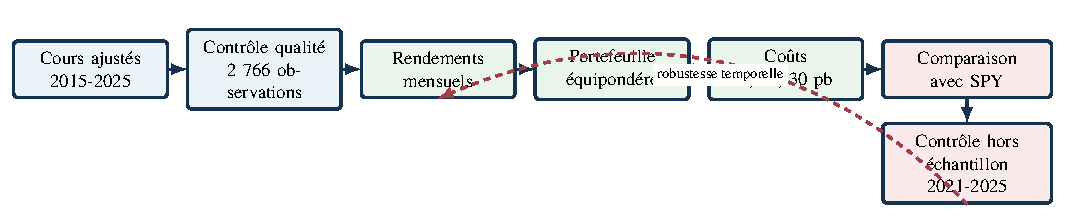
\includegraphics[width=\textwidth]{figures/schemas/protocole_experimental.pdf}
\caption{Déroulement du protocole expérimental et contrôle hors échantillon.}
\label{fig:protocole-experimental}
\end{figure}

\section{Limites de la méthode}

Le benchmark proposé constitue une première validation empirique du socle quantitatif, mais pas une évaluation complète d'un système agentique. Une telle évaluation nécessiterait un univers d'actifs, des données historiques propres, un protocole hors échantillon, une modélisation des coûts et des contraintes de liquidité. L'objectif est donc architectural et méthodologique : identifier les briques pertinentes, analyser leur rôle et proposer une architecture explicable.

Une autre limite concerne l'évolution rapide des dépôts GitHub. Les projets agentiques sont actifs, changent fréquemment d'API et peuvent modifier leur licence ou leur stratégie de maintenance. Toute décision d'adoption doit donc inclure une revue technique datée, une analyse de sécurité des dépendances et une validation juridique de la licence.

% Texte d'exemple du template conservé hors compilation.


\chapter{Architecture proposée et composants exécutés}\label{cap:architecture}

\section{Répartition des responsabilités}

J'ai retenu une règle : les métriques financières et les valeurs de portefeuille proviennent de fonctions déterministes. Dans la synthèse, LangGraph organise la lecture des résultats, les contrôles et la note DeepSeek. Dans l'allocation, un autre module transmet les indicateurs au LLM puis contrôle ses propositions avant toute transaction simulée. Aucun programme ne dispose d'un outil d'ordre réel.

La figure~\ref{fig:architecture-globale} décrit le dispositif proposé pour un desk plus complet. Les données, calculs, agents et validations y ont des responsabilités séparées. Les flèches représentent un passage d'état ; une sortie non conforme serait renvoyée au composant responsable.

\begin{figure}[H]
\centering
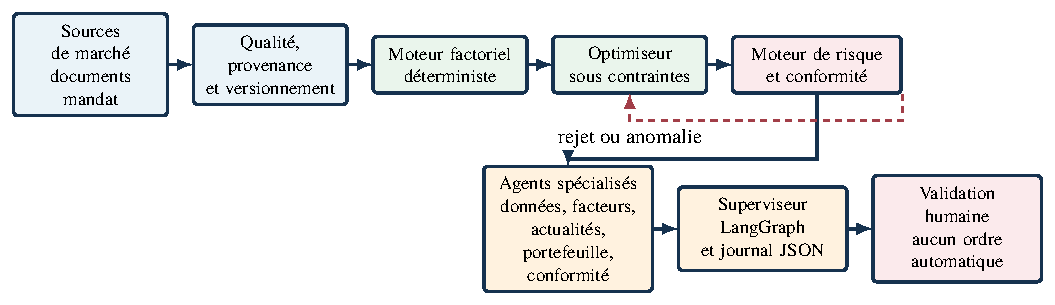
\includegraphics[width=\textwidth]{figures/schemas/architecture_globale.pdf}
\caption{Architecture cible séparant le socle quantitatif, les agents et la gouvernance.}
\label{fig:architecture-globale}
\end{figure}

\section{Rôles proposés et périmètre réalisé}

Les rôles du tableau~\ref{tab:agents-proposes} décrivent l'architecture cible : tous n'ont pas été exécutés. Les composants testés sont précisés après le tableau.

\begin{table}[H]
\centering
\caption{Rôles, permissions et limites des agents proposés.}
\label{tab:agents-proposes}
\scriptsize
\begin{adjustbox}{width=\textwidth}
\begin{tabular}{p{0.12\textwidth}p{0.20\textwidth}p{0.17\textwidth}p{0.18\textwidth}p{0.16\textwidth}p{0.17\textwidth}}
\toprule
\textbf{Agent} & \textbf{Mission} & \textbf{Outils autorisés} & \textbf{Sortie attendue} & \textbf{Interdictions} & \textbf{Conditions d'escalade} \\
\midrule
Données & Vérifier disponibilité, fraîcheur, provenance et cohérence. & APIs de données, contrôles qualité, logs. & Rapport de qualité et alertes. & Ne pas corriger silencieusement une donnée. & Donnée manquante, périmée ou incohérente. \\
Facteurs & Lancer les calculs et comparer les distributions. & Moteur déterministe, notebooks validés. & Scores, variations et anomalies. & Ne pas changer la formule ni les paramètres. & Rupture de distribution ou résultat non rejouable. \\
Actualités & Résumer nouvelles, résultats et événements macro. & OpenBB, flux autorisés, base RAG. & Synthèse sourcée et confiance. & Ne pas modifier les poids ni produire d'ordre. & Sources contradictoires ou absence de source. \\
Portefeuille & Proposer une allocation sous contraintes. & Optimiseur, mandat et coûts. & Poids cibles et attribution. & Ne pas contourner un rejet risque ou conformité. & Allocation infaisable ou contrainte violée. \\
Risque & Contrôler expositions, volatilité, drawdown et scénarios. & Moteur de risque, limites, stress tests. & Avis accepté, rejeté ou escaladé. & Ne pas relever lui-même une limite. & Limite franchie, modèle absent ou liquidité inconnue. \\
Conformité & Vérifier restrictions, documentation et séparation des rôles. & Référentiel de règles, listes, audit. & Validation ou blocage motivé. & Ne pas accorder d'exception implicite. & Règle inconnue, conflit ou trace incomplète. \\
Superviseur & Agréger les avis et préparer la revue humaine. & État complet, règles de délégation, journal. & Note de décision traçable. & Ne pas exécuter ni masquer un désaccord. & Désaccord, confiance faible ou intervention requise. \\
\bottomrule
\end{tabular}
\end{adjustbox}
\end{table}

Le workflow exécuté charge les fichiers, applique les gardes qualité et risque, puis associe un superviseur déterministe à la synthèse DeepSeek. Actualités et conformité restent proposées ; le rôle portefeuille est testé séparément dans l'extension d'allocation.

Dans le workflow de synthèse, le rapport qualité est lu après le backtest : une anomalie bloque l'accès au LLM. Le dépassement du seuil de turnover de 10\,\% ajoute une alerte d'escalade, sans interrompre la synthèse. Une sortie non conforme aux contrôles disponibles est rejetée et archivée ; le statut reste « à valider ». Les indicateurs de permission ne constituent pas une décision humaine enregistrée.

Le socle calcule rendements, poids après rendement, coûts, turnover et risque à partir de sources et paramètres identifiables, sans optimiseur institutionnel ni modèle de liquidité. Le dispositif complet prévoirait une validation humaine distincte du calcul et du contrôle qualité.

\section{Journal de décision et explicabilité}

Pour examiner une note, je repars du journal qui conserve les valeurs sources, les alertes et les permissions. Trois niveaux doivent être distingués : l'explication quantitative des calculs ; la trace des entrées, outils et règles de l'agent ; puis l'identité de la règle ou de la personne ayant validé la décision. Le texte libre demande un contrôle séparé de sa cohérence avec ces éléments.

L'extrait de la figure~\ref{fig:json-decision} provient du 30 novembre 2025. L'absence d'outil de modification des poids et d'envoi d'ordres se vérifie dans le code du workflow de synthèse ; les champs JSON en documentent la règle.

\begin{figure}[H]
\centering
\scriptsize
\begin{verbatim}
{
  "workflow": "langgraph_deterministic_supervisor",
  "date": "2025-11-30",
  "quality_ok": true,
  "risk_status": "a valider",
  "rebalance": {
    "factor_returns": {
      "Value": 0.0249981345118395,
      "Momentum": -0.0156164272534177,
      "Quality": 0.0090677798205325,
      "Low volatility": 0.0230736302539755
    },
    "net_return": 0.0103740219288315,
    "turnover": 0.0067574044008865,
    "transaction_cost": 6.757404400886513e-06,
    "target_weights": {
      "VLUE": 0.25, "MTUM": 0.25,
      "QUAL": 0.25, "USMV": 0.25
    }
  },
  "permissions": {
    "can_change_weights": false,
    "can_send_orders": false,
    "human_validation_required": true
  }
}
\end{verbatim}
\caption{Extrait réel du journal JSON produit par le prototype.}
\label{fig:json-decision}
\end{figure}

Les traces déterministes contiennent les valeurs, alertes et permissions. L'archive DeepSeek du 7 septembre 2026 ajoute le modèle et les identifiants de requête, mais pas les empreintes du prompt, des données ou le commit Git. Le code prévoit ces informations pour de nouvelles traces ; elles ne complètent pas rétroactivement l'archive. Aucune de ces sorties n'enregistre une approbation humaine effectivement réalisée.

\section{Allocation simulée et suivi des incidents}

L'extension suit une séquence explicite : indicateurs passés, proposition DeepSeek, validation indépendante, transaction simulée ou conservation des positions, puis valorisation quotidienne. Le modèle n'écrit jamais directement les quantités. Le code vérifie les poids, le turnover et les champs cités ; il revérifie les contraintes au cours d'exécution et finance les frais à partir du portefeuille.

Un rejet conserve les quantités et son motif est archivé, sans correction automatique ni nouvel appel. Le renvoi à un optimiseur avant revue humaine appartient à l'architecture proposée, pas à cette expérience. Le protocole et les résultats figurent respectivement aux sections~\ref{sec:protocole-allocation} et~\ref{sec:resultats-allocation}.

Un dispositif d'exploitation devrait suivre les citations invalides, échecs d'outils, désaccords, interventions humaines, latences et coûts, avec un responsable et une réaction définis pour chaque incident. Les seuils envisagés pour cette cible n'ont pas été calibrés sur le prototype. Les résultats mesurés de la collecte, ses rejets et ses limites sont discutés au chapitre~\ref{cap:discussion}.


\chapter{Discussion et analyse critique}\label{cap:discussion}
%--------------------------------------

\section{Apports de l'approche agentique}

L'approche agentique apporte une réponse crédible à plusieurs limites des chaînes quantitatives classiques. Une stratégie multifactorielle produit souvent des sorties numériques difficiles à contextualiser : scores, expositions, contraintes actives, turnover et attribution. Les agents peuvent transformer ces sorties en une note compréhensible, relier les mouvements du portefeuille à des événements de marché et signaler les cas où le modèle statistique semble en contradiction avec l'information qualitative.

Le deuxième apport est organisationnel. Une architecture multi-agents reproduit la séparation des responsabilités d'un desk : recherche, risque, conformité, exécution et supervision. Cette séparation rend le système plus auditable qu'un agent monolithique. Elle permet aussi de tester chaque agent séparément : exactitude des synthèses pour l'agent actualités, respect des limites pour l'agent risque, complétude documentaire pour l'agent conformité.

Le troisième apport concerne la mémoire. Des projets comme FinMem montrent qu'un agent peut conserver un historique structuré des événements et de ses propres décisions. Dans un contexte de marché, cette mémoire doit être contrôlée : elle peut aider à détecter les régimes récurrents, mais elle peut aussi renforcer des biais si elle n'est pas validée par des métriques objectives.

\section{Risques spécifiques}

Les risques spécifiques sont reliés à des contrôles, à des responsables et à des décisions observables. Cette présentation évite de traiter une faiblesse agentique comme un simple problème de rédaction.

\begin{table}[H]
\centering
\caption{Risques agentiques, contrôles et responsabilités.}
\label{tab:risques-agentiques}
\scriptsize
\begin{adjustbox}{width=\textwidth}
\begin{tabular}{p{0.16\textwidth}p{0.22\textwidth}p{0.20\textwidth}p{0.27\textwidth}p{0.11\textwidth}}
\toprule
\textbf{Risque} & \textbf{Exemple} & \textbf{Conséquence} & \textbf{Contrôle} & \textbf{Responsable} \\
\midrule
Hallucination & Source inexistante ou chiffre mal interprété. & Décision fondée sur une information fausse. & Récupération sourcée, validation des citations, blocage si source invalide. & Conformité \\
Surapprentissage narratif & Explication convaincante d'un signal non robuste. & Confusion entre récit et preuve financière. & Séparation temporelle, coûts, benchmark et tests de sensibilité. & Quant et risque \\
Permission excessive & Agent autorisé à modifier les poids ou à appeler l'exécution. & Action non validée et difficile à annuler. & Permissions minimales, outils déterministes et validation humaine. & IT et risque \\
Dépendance au modèle & Réponse différente après changement de version. & Décision non reproductible ou dérive de comportement. & Versionnement des modèles, prompts, données, outils et sorties. & Propriétaire IA \\
Désaccord non traité & Agents risque et portefeuille produisent des avis incompatibles. & Consensus artificiel et perte d'un signal d'alerte. & Conservation des avis, escalade et décision humaine explicite. & Superviseur \\
\bottomrule
\end{tabular}
\end{adjustbox}
\end{table}

\section{Explicabilité : trois niveaux}

\subsection{Explicabilité quantitative}

Elle relie la décision aux rendements, aux facteurs, aux pondérations, aux coûts, aux contraintes et aux métriques de risque. Les valeurs doivent provenir des sorties du moteur déterministe et pouvoir être recalculées avec la même version de données.

\subsection{Explicabilité agentique}

Elle décrit les sources consultées, les outils appelés, l'état parcouru, les règles appliquées, le niveau de confiance et les éventuels désaccords entre agents. Une synthèse ne peut être considérée comme fiable que si ses citations et ses entrées structurées sont vérifiables.

\subsection{Explicabilité de la décision finale}

Elle identifie l'avis du superviseur, la règle ou la personne qui a validé, modifié, rejeté ou différé la recommandation. Elle précise également si une permission d'exécution existait. Le journal JSON est donc l'élément de preuve ; la note en langage naturel en est l'interface de lecture.

\begin{figure}[H]
\centering
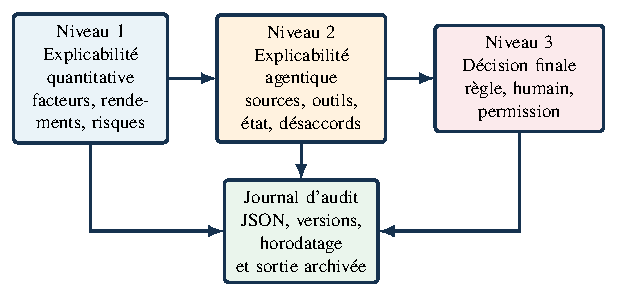
\includegraphics[width=\textwidth]{figures/schemas/explicabilite_trois_niveaux.pdf}
\caption{Trois niveaux d'explicabilité reliés au journal d'audit.}
\label{fig:explicabilite-trois-niveaux}
\end{figure}

\section{Positionnement des solutions GitHub}

Les solutions GitHub identifiées peuvent être positionnées sur une échelle de maturité.

Les frameworks comme LangGraph, AutoGen, CrewAI et Semantic Kernel sont matures pour orchestrer des workflows, mais ils ne connaissent pas le métier du trading. Ils sont adaptés à la couche agentique, pas au moteur financier.

Les plateformes comme Qlib, Lean, OpenBB, FinRL et Freqtrade sont utiles pour construire le socle quantitatif. Elles apportent données, backtesting, simulation ou environnement d'apprentissage. Elles ne garantissent pas l'explicabilité agentique, mais elles permettent de rendre les calculs reproductibles.

Les projets comme TradingAgents, FinRobot, FinMem et AI Hedge Fund sont les plus proches de l'intuition multi-agents. Leur valeur est exploratoire : ils montrent comment découper les rôles et produire des analyses financières. Leur faiblesse est le passage à l'échelle réglementaire : contrôle des données, validation indépendante, limites de risque, sécurité, audit et intégration à une infrastructure institutionnelle.

\section{Conditions minimales de mise en production}

Avant un déploiement réel, un système agentique de trading devrait satisfaire au minimum les conditions suivantes :
\begin{itemize}
    \item fonctionnement initial en mode observation, sans exécution automatique ;
    \item jeux de tests sur données historiques et scénarios extrêmes ;
    \item séparation stricte entre agents de recherche, agents de décision et outils d'exécution ;
    \item limites de risque codées hors LLM et impossibles à contourner par prompt ;
    \item registre d'audit complet et horodaté ;
    \item validation indépendante par risque, conformité et IT ;
    \item plan de repli en cas d'indisponibilité du modèle ou de dérive des sorties ;
    \item revue périodique des performances financières et des erreurs agentiques.
\end{itemize}

La trajectoire raisonnable est donc graduelle : assistant de recherche, assistant de reporting, assistant de revue de risque, puis assistant de recommandation supervisée. Le passage à une autonomie d'exécution ne devrait être envisagé qu'après une longue période de monitoring et seulement pour des stratégies à périmètre limité.

\section{Résultats du prototype expérimental}

Le prototype présenté au chapitre~\ref{cap:methodologie} fournit une première mesure du comportement d'une combinaison équipondérée de quatre sleeves factoriels. Les résultats sont comparés à l'ETF \texttt{SPY} sur la période février 2015-décembre 2025, qui correspond aux rendements mensuels calculés à partir des cours ajustés.

\begin{table}[H]
\centering
\caption{Résultats du prototype multifactoriel et du benchmark.}
\label{tab:resultats-backtest}
\scriptsize
\begin{tabular}{lrrrrrr}
\toprule
\textbf{Scénario} & \textbf{Rend. ann.} & \textbf{Vol. ann.} & \textbf{Sharpe} & \textbf{Drawdown} & \textbf{Valeur finale} & \textbf{Turnover mensuel} \cr
\midrule
SPY & 13,95\,\% & 14,96\,\% & 0,946 & -23,93\,\% & 411,73 & - \cr
Multifactoriel, 0 pb & 12,11\,\% & 14,17\,\% & 0,876 & -23,84\,\% & 345,38 & 1,26\,\% \cr
Multifactoriel, 10 pb & 12,10\,\% & 14,17\,\% & 0,875 & -23,86\,\% & 344,82 & 1,26\,\% \cr
Multifactoriel, 30 pb & 12,06\,\% & 14,17\,\% & 0,873 & -23,88\,\% & 343,69 & 1,26\,\% \cr
\bottomrule
\end{tabular}
\end{table}

Sur cette période, le benchmark \texttt{SPY} obtient le rendement annualisé le plus élevé et le meilleur ratio de Sharpe. Le portefeuille multifactoriel présente toutefois une volatilité et un drawdown légèrement inférieurs. Les coûts de transaction modifient peu le résultat dans cette configuration, car le turnover mensuel moyen reste limité.

Une vérification temporelle est également effectuée sur la période hors échantillon 2021-2025. À 10 points de base, le multifactoriel obtient un rendement annualisé de 11,45\,\%, une volatilité de 14,37\,%, un Sharpe de 0,816 et une valeur finale de 170,33. Sur la même période, SPY atteint 14,60\,%, 15,14\,%, 0,965 et 195,39. Cette comparaison confirme la prudence de l'interprétation : le prototype ne montre pas de supériorité du multifactoriel, mais fournit une base reproductible pour tester l'architecture.

\begin{table}[H]
\centering
\caption{Contrôle hors échantillon sur la période 2021-2025.}
\label{tab:resultats-oos}
\scriptsize
\begin{tabular}{lrrrrrr}
\toprule
\textbf{Scénario} & \textbf{Rend. ann.} & \textbf{Vol. ann.} & \textbf{Sharpe} & \textbf{Drawdown} & \textbf{Valeur finale} & \textbf{Turnover mensuel} \\
\midrule
SPY & 14,60\,\% & 15,14\,\% & 0,965 & -23,93\,\% & 195,39 & - \\
Multifactoriel, 10 pb & 11,45\,\% & 14,37\,\% & 0,816 & -23,86\,\% & 170,33 & 1,53\,\% \\
\bottomrule
\end{tabular}
\end{table}

\begin{figure}[H]
    \centering
    
\includegraphics[width=0.94\textwidth]{figures/cumulative_wealth.png}
    \caption{Évolution d'un investissement initial de 100 unités.}
    \label{fig:cumulative-wealth}
\end{figure}

\begin{figure}[H]
    \centering
    
\includegraphics[width=0.94\textwidth]{figures/drawdown.png}
    \caption{Drawdown du benchmark et des portefeuilles multifactoriels.}
    \label{fig:drawdown}
\end{figure}

Ces résultats ne prouvent donc pas la supériorité financière de la stratégie multifactorielle. Ils montrent plutôt l'intérêt d'un socle quantitatif reproductible auquel un agent peut être relié. L'agent pourrait recevoir ces sorties structurées afin de produire une note de décision, mais il ne doit ni recalculer les métriques ni modifier les pondérations sans règle déterministe et validation humaine.

\section{Démonstration de la couche agentique}

Le module \texttt{agent\_workflow.py} exécute désormais ce scénario avec LangGraph. Les deux exemples du 30 novembre et du 31 décembre 2025 sont générés à partir des sorties structurées du rééquilibrage, sans nouvel appel de données et sans accès aux ordres. Le premier exemple correspond au 30 novembre 2025 : les rendements de VLUE, MTUM, QUAL et USMV sont respectivement de +2,50\,\%, -1,56\,\%, +0,91\,\% et +2,31\,\%. Le rendement net du portefeuille est de +1,04\,\% pour un turnover de 1,35\,\%. La note conclut que la hausse de VLUE et USMV compense la baisse de MTUM et recommande de conserver les pondérations cibles de 25\,\%, sous réserve d'une validation humaine.

Le second exemple correspond au 31 décembre 2025 : VLUE progresse de +2,90\,\%, MTUM de +0,29\,\%, QUAL de +0,58\,\% et USMV recule de -0,82\,\%. Le rendement net du portefeuille atteint +0,74\,\% pour un turnover de 1,07\,\%. La note identifie VLUE comme principal facteur favorable, signale la contribution négative de USMV et ne propose aucun ajustement exceptionnel.

Ces notes sont comparées aux fichiers de sortie du prototype selon quatre critères : fidélité aux chiffres, complétude, respect des permissions et explicitation des limites. Le résultat est observable sur les deux exécutions ; cette évaluation manuelle constitue une première vérification qualitative et non une mesure statistique de la qualité d'un agent.

\begin{table}[H]
\centering
\caption{Évaluation des deux démonstrations agentiques.}
\label{tab:evaluation-agent}
\scriptsize
\begin{adjustbox}{width=\textwidth}
\begin{tabular}{p{0.15\textwidth}p{0.18\textwidth}p{0.18\textwidth}p{0.18\textwidth}p{0.20\textwidth}p{0.08\textwidth}}
\toprule
\textbf{Date} & \textbf{Fidélité aux chiffres} & \textbf{Complétude} & \textbf{Permissions} & \textbf{Limites explicitées} & \textbf{Résultat} \\
\midrule
30/11/2025 & Conforme : rendements, net et turnover cohérents avec le JSON. & Conforme : facteurs favorables et défavorables identifiés. & Conforme : aucun changement de poids ni ordre. & Conforme : validation humaine et limites du moteur signalées. & Conforme \\
31/12/2025 & Conforme : rendements, net et turnover cohérents avec le JSON. & Conforme : VLUE et USMV sont correctement contextualisés. & Conforme : aucun changement de poids ni ordre. & Conforme : validation humaine et limites du moteur signalées. & Conforme \\
\bottomrule
\end{tabular}
\end{adjustbox}
\end{table}

\section{Synthèse}

L'approche agentique est pertinente pour un desk multifactoriel si elle est conçue comme une architecture de coordination et d'explicabilité. Elle devient fragile si elle est présentée comme un substitut au modèle quantitatif ou au contrôle humain. Le meilleur compromis consiste à combiner des agents spécialisés avec des moteurs déterministes, des règles non contournables et un journal de décision exploitable par un auditeur.

% Texte d'exemple du template conservé hors compilation.


\chapter{Conclusion}\label{cap:conclusion}

\section{Ce que je retiens du prototype}

J'ai examiné les contrôles des synthèses et des allocations proposées par le LLM.

Le backtest m'a fourni le socle de cette comparaison : l'équipondération des quatre ETF reste derrière SPY en rendement annualisé, après frais de transaction. Le contrôle sur 2021--2025 conserve ce classement. J'y vois un cas reproductible pour l'étude de la couche agentique, sans supériorité financière du multifactoriel.

Les synthèses DeepSeek satisfont les contrôles automatisés, mais trois altérations construites passent aussi le validateur : coût inexact, citation inexistante et recommandation contradictoire. Ces essais m'ont conduit à examiner ce que le validateur laisse passer, au-delà du taux d'acceptation. La fiabilité du texte et son utilité pour un analyste demanderaient également une lecture indépendante.

Dans l'extension d'allocation, DeepSeek termine derrière l'équipondération et l'inverse volatilité, après frais de transaction. Sur 56 propositions, 34 sont rejetées, surtout pour dépassement du turnover. Je retiens ici l'utilité du contrôle, qui bloque des propositions incorrectes. Le rendement obtenu dépend aussi de ces rejets et de la conservation des positions qu'ils déclenchent : il évalue l'ensemble du dispositif.

Ce travail m'a ainsi conduit à déplacer la question initiale : l'enjeu n'est pas seulement de savoir ce qu'un LLM peut produire pour un desk, mais surtout ce que le système est capable de vérifier avant d'utiliser cette production.

\section{Limites de portée}

Le PnL d'allocation reste rétrospectif : les indicateurs sont coupés dans le temps, mais le préentraînement peut contenir les événements étudiés. Une seule trajectoire a été collectée et les données ne sont pas disponibles dans leurs versions historiques point-in-time. Le replay et les 46 tests établissent la cohérence technique, sans démontrer la généralisation financière.

Je conserve également une réserve sur le bilan des coûts : le PnL exclut l'API, l'infrastructure et le travail humain. Les 66\,014 jetons connus, auxquels peut s'ajouter l'usage de la requête interrompue, documentent une consommation partielle. La facture, le coût total d'exploitation et les gains éventuels de temps restent à mesurer.

\section{Deux suites prioritaires}

Je renforcerais d'abord la fiabilité des sorties : tolérances adaptées aux champs, citations exactes et cohérence du texte pour les notes ; choix parmi des portefeuilles déjà admissibles pour l'allocation. Ce dernier dispositif serait comparé à une règle utilisant les mêmes indicateurs, selon un protocole défini avant observation des rendements puis suivi prospectivement.

Je comparerais ensuite les notes auprès d'analystes sur plusieurs dates, en faisant varier l'ordre de présentation. L'exactitude des réponses, la détection des alertes et le temps nécessaire seraient rapprochés des coûts API et de revue, pour évaluer la valeur pratique de cette intégration.


\newpage

%---------------------------------------------------------------------------
% Bibliographie
\addcontentsline{toc}{chapter}{Bibliographie}
\bibliographystyle{apalike-fr} % Variante locale : liaisons entre auteurs en français
\bibliography{biblio.bib}       % Carga las referencias desde el archivo biblio.bib y crea la sección de Bibliografía
%---------------------------------------------------------------------------
% Annexes
\appendix
\clearpage
\renewcommand{\thechapter}{\Roman{chapter}}
\chapter{Matrice des solutions GitHub}\label{annexe:github}

\section{Solutions recommandées pour l'étude comparative}

Cette annexe synthétise les dépôts les plus directement exploitables pour transformer l'état de l'art en cartographie exploitable. Les URLs et licences doivent être revérifiées avant tout usage institutionnel.

\begin{table}[H]
\centering
\caption{Matrice de sélection des dépôts GitHub.}
\label{tab:annexe-github}
\scriptsize
\begin{adjustbox}{width=\textwidth}
\begin{tabular}{p{0.17\textwidth}p{0.20\textwidth}p{0.31\textwidth}p{0.26\textwidth}}
\toprule
\textbf{Dépôt} & \textbf{Rôle} & \textbf{Usage conseillé} & \textbf{Précaution} \\
\midrule
LangGraph & Orchestration & Construire le graphe d'étapes : ingestion, calcul, analyse, risque, conformité, supervision. & Versionner les états et imposer des sorties structurées. \\
AutoGen & Collaboration multi-agents & Prototyper des conversations entre agents analystes et contrôleurs. & Encadrer strictement les permissions d'outils. \\
CrewAI & Agents par rôles & Démontrer rapidement un workflow de recherche financière. & Ajouter logs, contrôles et tests avant usage sérieux. \\
Semantic Kernel & Intégration entreprise & Connecter agents, fonctions et plugins dans un environnement Microsoft. & Ne fournit pas de modèle financier prêt à l'emploi. \\
Qlib & Recherche quantitative & Calculer signaux, entraîner modèles, backtester des stratégies. & Adapter données, coûts et contraintes au mandat réel. \\
Lean & Backtesting et exécution & Simuler et exécuter des stratégies multi-actifs. & Garder l'exécution sous règles déterministes. \\
OpenBB & Données et recherche & Alimenter un agent de veille et de synthèse financière. & Vérifier les licences des fournisseurs de données. \\
FinRL / FinRL-Meta & Agents RL financiers & Comparer LLM agents et RL sur environnements de marché. & Risque fort de surapprentissage. \\
TradingAgents & Multi-agents trading & Inspirer l'équipe d'agents : analystes, trader, risque. & Prototype de recherche, non suffisant pour production régulée. \\
FinRobot & Agents financiers LLM & Automatiser recherche actions et valorisation. & Compléter par un moteur quantitatif et des contrôles. \\
FinMem & Mémoire agentique & Étudier l'impact d'une mémoire structurée sur les décisions. & Valider empiriquement la robustesse hors échantillon. \\
AI Hedge Fund & Démonstrateur pédagogique & Montrer la division des rôles dans un fonds simulé. & Preuve de concept, pas outil de trading réel. \\
\bottomrule
\end{tabular}
\end{adjustbox}
\end{table}
\section{Due diligence des dépôts au 30 août 2026}

Les informations ci-dessous ont été relevées sur les dépôts publics et l'API GitHub le 30 août 2026. La date de dernier push renseigne l'activité observée, mais ne garantit ni la maintenance ni l'aptitude à un usage institutionnel. Le propriétaire public est indiqué ; le nombre de mainteneurs actifs n'est pas assimilé au nombre de contributeurs.

\begin{table}[H]
\centering
\caption{Grille de due diligence des briques sélectionnées.}
\label{tab:due-diligence}
\scriptsize
\begin{adjustbox}{width=\textwidth}
\begin{tabular}{p{0.14\textwidth}p{0.13\textwidth}p{0.14\textwidth}p{0.20\textwidth}p{0.16\textwidth}p{0.18\textwidth}}
\toprule
\textbf{Dépôt} & \textbf{Licence} & \textbf{Dernier push} & \textbf{Docs et tests} & \textbf{Sécurité} & \textbf{Avis provisoire} \\
\midrule
LangGraph \citep{githubLangGraph} & MIT & 30/08/2026 & README, docs ; tests à inspecter & Politique présente & Orchestration active ; audit dépendances. \\
Qlib \citep{githubQlib} & MIT & 23/07/2026 & docs, tests & SECURITY.md & Brique quantitative documentée. \\
Lean \citep{githubLean} & Apache-2.0 & 28/08/2026 & README, Tests & À vérifier & Moteur actif ; audit des données. \\
OpenBB \citep{githubOpenBB} & AGPLv3* & 30/07/2026 & README, pytest.ini & SECURITY.md & Licence à valider juridiquement. \\
TradingAgents \citep{githubTradingAgents} & Apache-2.0 & 30/08/2026 & README, tests & À vérifier & Prototype multi-agents. \\
FinRobot \citep{githubFinRobot} & Apache-2.0 & 23/08/2026 & README, test\_module.py & À vérifier & Démonstrateur financier. \\
FinRL \citep{githubFinRL} & MIT & 13/07/2026 & docs, unit\_tests & À vérifier & RL ; surapprentissage à contrôler. \\
Freqtrade \citep{githubFreqtrade} & GPL-3.0 & 27/08/2026 & docs, tests & À vérifier & Bot crypto ; périmètre différent. \\
\bottomrule
\end{tabular}
\end{adjustbox}
\end{table}

\noindent * Le README OpenBB déclare AGPLv3, tandis que l'API GitHub renvoie \texttt{NOASSERTION}; une vérification juridique est donc obligatoire. Le fichier structuré complet est archivé dans \texttt{github\_due\_diligence.json}.


\section{Statut d'utilisation dans le mémoire}

La due diligence est complétée par un statut d'utilisation. Cette distinction indique si une brique a été exécutée dans le prototype, utilisée comme référence pour la conception ou seulement étudiée dans la cartographie.

\begin{table}[H]
\centering
\caption{Statut des solutions dans le travail réalisé.}
\label{tab:statut-utilisation}
\scriptsize
\begin{adjustbox}{width=\textwidth}
\begin{tabular}{p{0.22\textwidth}p{0.23\textwidth}p{0.43\textwidth}}
\toprule
\textbf{Dépôt} & \textbf{Statut} & \textbf{Rôle dans le travail} \\
\midrule
LangGraph & Utilisé dans le prototype & Workflow déterministe de lecture des sorties quantitatives, génération des notes et contrôle des permissions. \\
Qlib & Référence étudiée & Comparaison pour la recherche quantitative et le backtesting ; non branché au calcul final. \\
Lean & Référence comparative & Exemple de moteur multi-actifs pour une évolution future du socle. \\
OpenBB & Référence étudiée & Brique étudiée pour la veille et la provenance des données ; non branchée au prototype. \\
TradingAgents & Étudié, non exécuté & Référence pour la séparation des rôles dans une architecture multi-agents financière. \\
FinRobot & Étudié, non exécuté & Référence pour les assistants de recherche et d'analyse financière. \\
FinRL & Étudié, non retenu & Solution RL documentée, hors périmètre du prototype ETF équipondéré. \\
Freqtrade & Étudié, hors périmètre principal & Brique crypto utile pour comparaison, mais non adaptée au protocole retenu. \\
\bottomrule
\end{tabular}
\end{adjustbox}
\end{table}

\section{Combinaison minimale}

Pour une étude de master réaliste, la combinaison suivante est suffisante :
\begin{itemize}
    \item LangGraph pour imposer un workflow auditable ;
    \item Qlib ou Lean pour calculer et backtester les signaux ;
    \item OpenBB pour alimenter la veille et les données financières ;
    \item un agent de synthèse pour produire la note de décision ;
    \item un registre JSON ou base SQL pour stocker chaque appel d'outil, donnée et validation.
\end{itemize}

Cette combinaison évite de dépendre d'un seul dépôt. Elle permet aussi de remplacer progressivement les composants : un moteur de risque interne peut remplacer une bibliothèque open source, un modèle LLM privé peut remplacer un modèle externe, et les règles de conformité peuvent être intégrées sous forme de fonctions déterministes.

% Texte d'exemple du template conservé hors compilation.

\chapter{Reproduction de l'expérience d'allocation}\label{ann:allocation}

L'expérience du 12 septembre 2026 est conservée dans \path{results/allocation_experiment/}. Le code, le prompt et les données utilisés sont identifiés par les empreintes de \fichiergithub{results/allocation_experiment/deepseek/report.json}{deepseek/report.json}. Les réponses restent consultables dans \fichiergithub{results/allocation_experiment/deepseek_decisions.json}{deepseek_decisions.json}. La reproduction locale ne nécessite ni clé API ni connexion réseau.

\section{Fichiers et vérifications}

\begin{description}
\item[Propositions et exécution :] \fichiergithub{results/allocation_experiment/deepseek/decisions.json}{deepseek/decisions.json} contient les entrées, propositions, quantités avant/après, dates d'exécution, frais et rejets des trois politiques.
\item[Valeurs et indicateurs :] \path{deepseek/equity.csv}, \path{deepseek/metrics.csv} et \path{yearly_returns.csv} fournissent les séries et résultats numériques.
\item[Essais techniques :] \fichiergithub{results/allocation_experiment/technical_pilot_default_thinking.json}{technical_pilot_default_thinking.json} conserve les quatre tentatives précédant la campagne corrigée ; elles ne sont pas fusionnées avec ses 56 décisions.
\item[Audit :] \fichiergithub{results/allocation_experiment/AUDIT.json}{AUDIT.json} conserve les écarts comptables, l'identité du replay et le contrôle des 31 fichiers antérieurs. Le manifeste correspondant est \fichiergithub{results/allocation_experiment/original_inputs_sha256.json}{original_inputs_sha256.json}.
\item[Documentation :] \fichiergithub{results/allocation_experiment/PROTOCOLE.md}{PROTOCOLE.md} et \fichiergithub{results/allocation_experiment/ANALYSE.md}{ANALYSE.md} détaillent conventions, résultats et limites.
\end{description}

\section{Commandes de reproduction sans appel API}

Depuis la racine du projet, la commande suivante relit les réponses archivées et calcule les positions :

\begin{quote}\small\ttfamily
experience/.venv/bin/python agent\_allocation\_backtest.py\\
\hspace*{1em}--mode replay --start 2021-05-01\\
\hspace*{1em}--archive \href{https://github.com/AbouOpenSource/projet-end-master/blob/be691b42772e9d223b1304fae597ba13ac62d505/results/allocation_experiment/deepseek_decisions.json}{results/allocation\_experiment/deepseek\_decisions.json}\\
\hspace*{1em}--max-output-tokens 3000\\
\hspace*{1em}--output results/allocation\_experiment/replay
\end{quote}
Les lignes sont présentées séparément pour la lecture ; la commande s'exécute sur une seule ligne. Les paramètres de coûts et de fin de période prennent leurs valeurs par défaut, 10 points de base et le 31 décembre 2025. Toute différence de contexte par rapport à une requête archivée interrompt le replay.

La vérification comptable et la suite de tests s'exécutent ensuite avec :
\begin{quote}\small\ttfamily
experience/.venv/bin/python analyze\_allocation\_results.py\\[0.3em]
experience/.venv/bin/python -m pytest -q
\end{quote}

Le mode \texttt{live}, décrit dans le \href{https://github.com/AbouOpenSource/projet-end-master/blob/be691b42772e9d223b1304fae597ba13ac62d505/README.md}{README}, nécessite une clé et un budget explicite. Il réutilise les dates de son archive et compte toutes les tentatives, y compris les interruptions. Rejouer les archives n'envoie pas de nouvel appel ; une nouvelle expérience avec un autre prompt ou d'autres contraintes doit utiliser une archive distincte et un budget identifié.

%---------------------------------------------------------------------------
\end{document}
